% --- Osnovna konfiguracija dokumenta ---
\documentclass[12pt, oneside, a4paper, hidelinks]{report}

% --- Kodiranje i jezik ---
\usepackage[utf8]{inputenc}
\usepackage[T1]{fontenc}
\usepackage[croatian]{babel}
\usepackage{cmap}
\usepackage{csquotes}

% --- Font ---
%\usepackage{lmodern}
\usepackage{newtx}

% --- Margine i raspored stranice ---
\newcommand{\mybindingoffset}{0.2in}
\newcommand{\myhalfbindingoffset}{0.1in}
\usepackage[
bindingoffset=\mybindingoffset,
left=1in, right=1in,
top=1in, bottom=1in,
headsep=.25in, footskip=.25in
]{geometry}

% --- Razmak i odlomci ---
\usepackage{setspace}
\linespread{1}
\setlength{\parskip}{0.5em}
\setlength{\parindent}{0pt}

% --- Zaglavlja i podnožja ---
\usepackage{fancyhdr}
\pagestyle{fancy}

% --- Boje ---
\usepackage{xcolor}

% --- Grafika i vizualizacija ---
\usepackage{graphicx}
\usepackage{float}
\usepackage{rotating}
\usepackage{pdflscape}
\usepackage{pdfpages}
\usepackage{tikz}

% --- Tablice i rasporedi ---
\usepackage{tabularx}
\newcolumntype{C}{>{\centering\arraybackslash}X}
\usepackage{multirow}
\usepackage{multicol}
\usepackage{booktabs}

% --- Naslovi i opisi ---
\usepackage[labelsep=period]{caption}
\captionsetup[table]{skip=0pt, singlelinecheck=off}
\usepackage{subcaption}

% --- Popisi i jednadžbe ---
\usepackage{enumitem}
\usepackage{subeqnarray}
\usepackage{chngcntr}
\counterwithout{equation}{chapter}

% --- Hiperveze ---
\usepackage[unicode]{hyperref}

% --- Metapodaci i makroi ---
\newcommand{\mytitle}{Naslov diplomskog rada}
\newcommand{\myauthor}{Ime i prezime}
\newcommand{\myabstract}{Na hrvatskom jeziku do 300 riječi.}
\newcommand{\mykeywords}{ključna riječ 1, ključna riječ 2, ključna riječ 3, ključna riječ 4, ključna riječ 5}

\title{\mytitle}
\author{\myauthor}
\date{2025.}

% --- PDF/A Metapodaci ---
%\begin{filecontents}[force]{\jobname.xmpdata}
%	\Author{\myauthor}
%	\Title{\mytitle}
%	\Language{hr}
%	\Keywords{ključna riječ 1\sep ključna riječ 2\sep ključna riječ 3\sep ključna riječ 4\sep ključna riječ 5}
%	\Subject{\myabstract}
%	\Date{2025-01-01}
%	\PublicationType{masterthesis}
%	\Copyrighted{true}
%	\Copyright{CC BY}
%   \CopyrightURL{https://creativecommons.org/licenses/by/4.0/}
%%	\Source{https://repozitorij.geof.unizg.hr/}
%%	\URLlink{https://repozitorij.geof.unizg.hr/}
%\end{filecontents}
%\usepackage[a-2b]{pdfx}

% --- Bibliografija ---
\usepackage[backend=biber,style=apa,defernumbers=true]{biblatex}
\addbibresource{PopisLiterature.bib}
\DeclareLanguageMapping{croatian}{croatian-apa}

% Prilagodba separatora u citatima
\DeclareDelimAlias{finalnamedelim}{finalnamedelim:apa:cite}
\DeclareDelimAlias{multinamedelim}{multinamedelim:apa:cite}
\DeclareDelimFormat{finalnamedelim:apa:cite}{\addspace i\space}
\DeclareDelimFormat{multinamedelim:apa:cite}{\addcomma\space}

% Formatiranje broja reference za URL-ove
\DeclareFieldFormat{labelnumber}{#1}

% Prilagodba citiranja URL-a
\renewbibmacro*{cite}{%
	\ifkeyword{url}
	{\printtext[bibhyperref]{\textsc{URL}~\printfield{labelnumber}}}
	{\printnames{labelname}\addcomma\space\printfield{year}\unskip}%
}

% Okruženje za bibliografiju s URL-ovima
\defbibenvironment{bibliographyURL}
{\list
	{\printtext[labelnumberwidth]{\textsc{URL}~\printfield{labelnumber}.}}
	{\setlength{\labelwidth}{\labelnumberwidth}
		\setlength{\leftmargin}{\labelwidth}
		\setlength{\labelsep}{\biblabelsep}
		\addtolength{\leftmargin}{\labelsep}
		\setlength{\itemsep}{\bibitemsep}
		\setlength{\parsep}{\bibparsep}}
	\renewcommand*{\makelabel}[1]{\hss##1}}
{\endlist}
{\item}

% Prilagodba prikaza online izvora (URL i redovni online izvori)
\DeclareBibliographyDriver{online}{%
	\ifkeyword{url}{%
		\printtext[labelnumberwidth]%
		\addspace
		\printfield{title}\addcolon\addspace
		\printfield{url}%
		\setunit*{\addspace}%
		\space
		\iffieldundef{urlyear}{}{%
			\mkbibparens{%
				\stripzeros{\thefield{urlday}}.%
				\stripzeros{\thefield{urlmonth}}.%
				\thefield{urlyear}.%
			}%
		}%
	}{%
		\printnames{author}%
		\addspace
		(\printfield{year}%
		\iffieldundef{month}{}{, \mkbibmonth{\thefield{month}}}%
		\iffieldundef{day}{}{~\thefield{day}}%
		).\space
		\textit{\printfield{title}}.%
		\iffieldundef{organization}{}{ \printfield{organization}.}%
		\setunit{\addspace}%
		\space
		\url{\thefield{url}}%
	}%
	\finentry
}

% --- Putanja za slike ---
\graphicspath{{./Slike}}

% --- Sadržaj i naslovi ---
\usepackage{titletoc}
\usepackage{tocloft}
\usepackage{titlesec}
\usepackage{lastpage}

% Prilagodba sadržaja
\renewcommand{\cftchapfont}{\normalfont}
\renewcommand{\cftchappagefont}{\normalfont}
\renewcommand{\cftchapleader}{\cftdotfill{\cftdotsep}}
\renewcommand{\cftdotsep}{1}

\setlength{\cftbeforechapskip}{8pt}

% Formatiranje naslova
\titleformat{\chapter}[block]{\normalfont\Large\bfseries}{\hspace{0em}}{0em}{\MakeUppercase}
\titlespacing*{\chapter}{0pt}{-12pt}{12pt}

\titleformat{\section}[block]{\normalfont\bfseries}{\thesection}{1em}{}
\titlespacing*{\section}{0pt}{18pt}{12pt}

\titleformat{\subsection}[block]{\normalfont\bfseries}{\thesubsection}{1em}{}
\titlespacing*{\subsection}{0pt}{12pt}{6pt}

% Format naslova popisa slika i tablica
\renewcommand{\cftloftitlefont}{\normalfont\Large\bfseries\MakeUppercase}
\renewcommand{\cftlottitlefont}{\normalfont\Large\bfseries\MakeUppercase}
\setlength{\cftbeforeloftitleskip}{3pt}
\setlength{\cftafterloftitleskip}{19pt}
\setlength{\cftbeforelottitleskip}{3pt}
\setlength{\cftafterlottitleskip}{19pt}

% Format brojeva slika i tablica
\setlength{\cftfigindent}{0em}
\renewcommand{\cftfigpresnum}{Slika }
\renewcommand{\cftfigaftersnum}{.}
\setlength{\cftfignumwidth}{5em}

\setlength{\cfttabindent}{0em}
\renewcommand{\cfttabpresnum}{Tablica }
\renewcommand{\cfttabaftersnum}{.}
\setlength{\cfttabnumwidth}{6em}

\begin{document}
	% --- Naslovna stranica ---
	\pagenumbering{Roman}
	\begin{titlepage}
		\begin{center}
			
\includegraphics[width=1in]{Logo_GEOF}\\
			\large\textbf{\MakeUppercase{Sveučilište u Zagrebu\\Geodetski fakultet}}
			\vfill
			
			\Large{\myauthor}\\
			\vspace{1in}
			\LARGE\textbf{\MakeUppercase{\mytitle}}\\
			\vspace{1in}
			\Large{Diplomski rad}\\
			\vfill
			
			\large{Zagreb, 2025.}
		\end{center}
	\end{titlepage}
	
	% --- Izjava o izvornosti ---
	\newpage
	\fancyhead{}
	\thispagestyle{empty}
	\renewcommand{\headrulewidth}{0pt}
	\setcounter{page}{2}
	\newgeometry{bindingoffset=\mybindingoffset, left=1.5in, right=1.5in, top=1.2in, bottom=1in, footskip=.25in}
	
	\newcommand{\backgroundpdf}{
		\begin{tikzpicture}[remember picture, overlay]
			\node[anchor=center, xshift=\myhalfbindingoffset] at (current page.center)
			{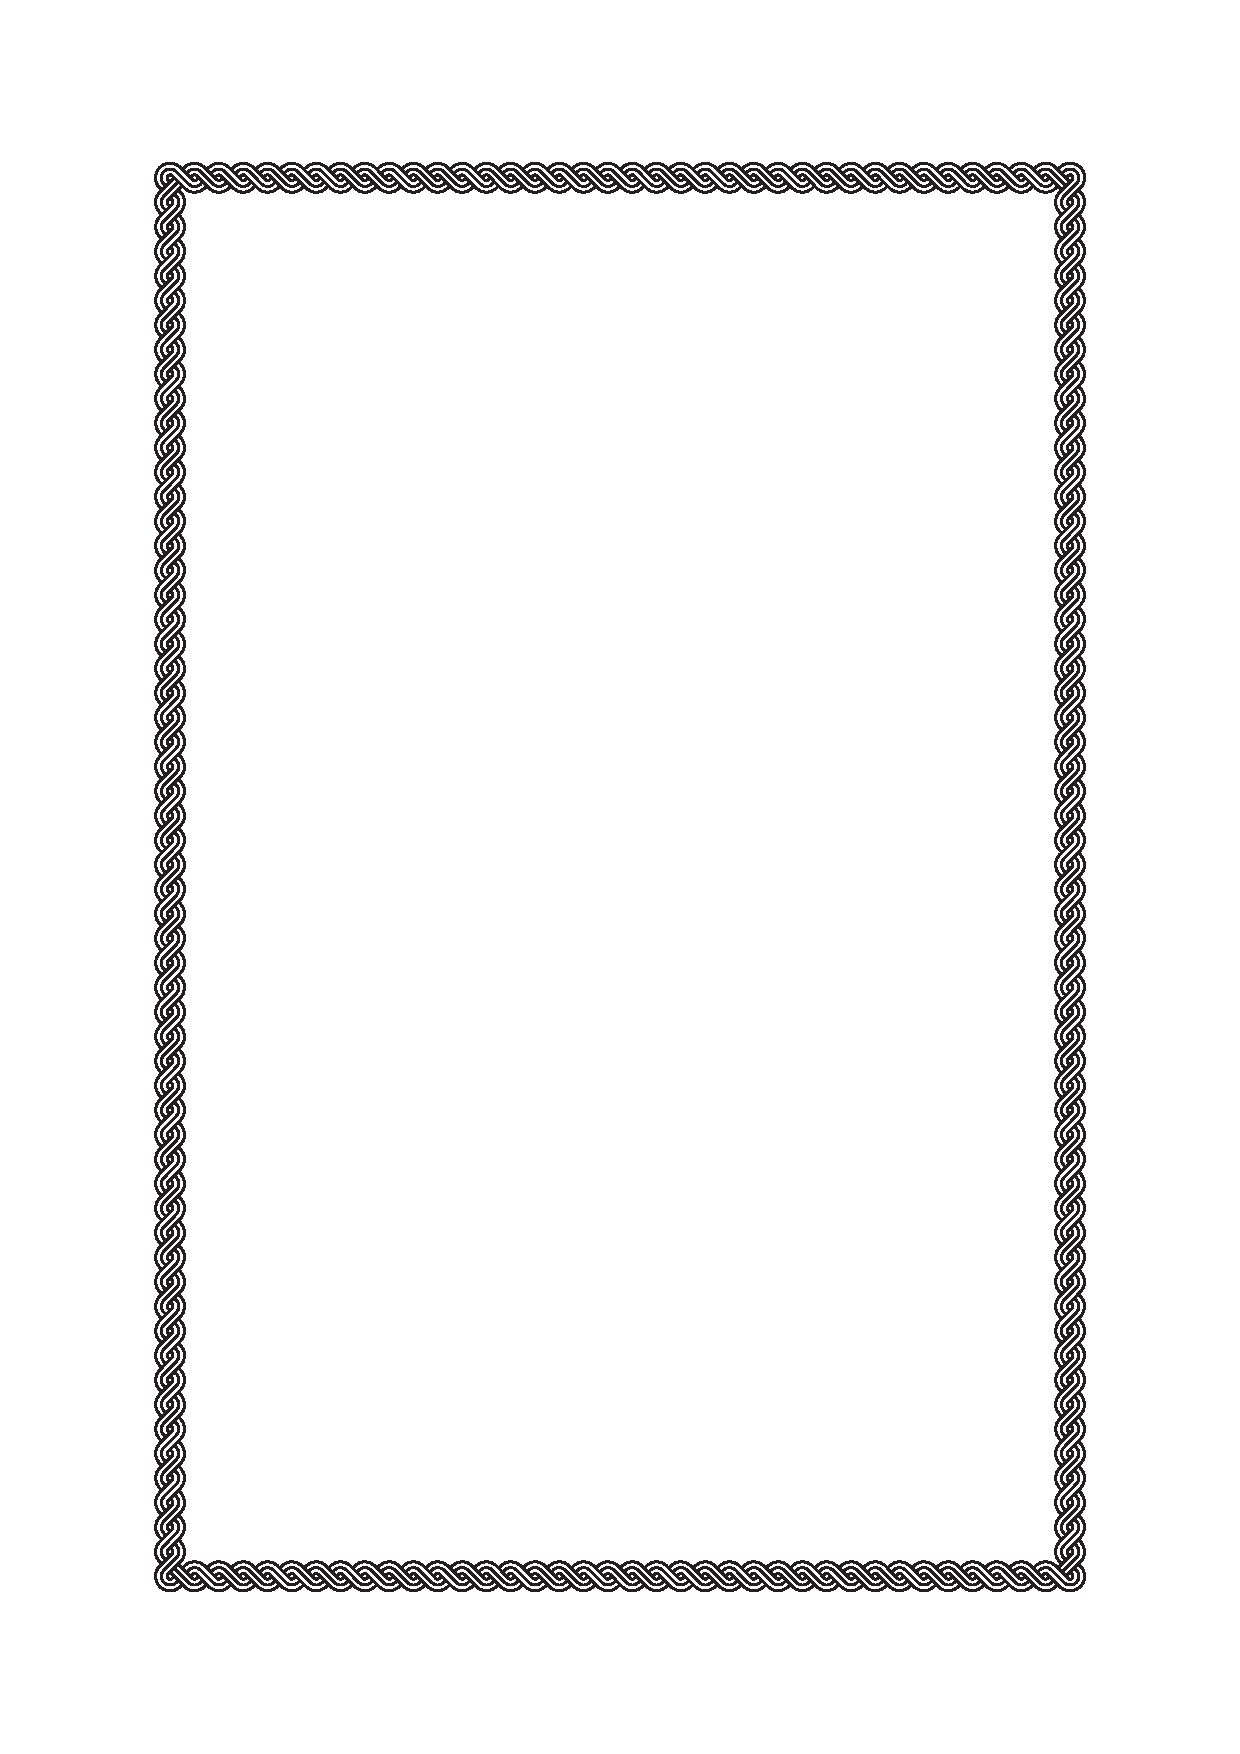
\includegraphics[width=\paperwidth]{Pleter.pdf}};
		\end{tikzpicture}
	}
	\backgroundpdf
	
	\begin{center}
		\large\textbf{\MakeUppercase{Sveučilište u Zagrebu\\Geodetski fakultet}}\\
		\vspace{.3in}
		
\includegraphics[width=1in]{Logo_GEOF}
	\end{center}
	\vspace{.5in}
	
	\noindent
	Na temelju članka 19. Etičkog kodeksa Sveučilišta u Zagrebu i Odluke br. 1\_349\_11 Fakultetskog vijeća Geodetskog fakulteta Sveučilišta u Zagrebu, od 26.10.2017. godine (klasa: 643-03/16-07/03), uređena je obaveza davanja „Izjave o izvornosti“ diplomskog rada koji se vrednuju na diplomskom studiju geodezije i geoinformatike, a u svrhu potvrđivanja da je rad izvorni rezultat rada studenata te da taj rad ne sadržava druge izvore osim onih koji su u njima navedeni.
	\vspace{.5in}
	
	\begin{center}
		\large\textbf{\MakeUppercase{izjavljujem}}\\
	\end{center}
	\vspace{.5in}
	
	\noindent
	Ja, \textbf{\myauthor}, (JMBAG: XXXXXXXXXX), rođen dana DD.MM.YYYY. u Naziv mjesta, izjavljujem da je moj diplomski rad izvorni rezultat mojeg rada te da se u izradi tog rada nisam koristio drugim izvorima osim onih koji su u njemu navedeni.
	\vspace{.8in}
	
	\noindent
	U Zagrebu, dana DD. mjesec 2025. \hfill \rule{2in}{.4pt}
	\begin{flushright}
		\textit{Potpis studenta / studentice}
	\end{flushright}
	
	% --- Tablica o diplomskom radu ---
	\newpage
	\fancypagestyle{plain}{
		\fancyhf{}
		\fancyfoot[R]{\small \thepage}
	}
	\restoregeometry
	\fancyhf{}
	\fancyfoot[R]{\small \thepage}
	\begin{table}[H]
		\centering
		\renewcommand{\arraystretch}{1.5}
		\begin{tabular}{|m{0.45\textwidth}|m{0.49\textwidth}|} 
			\hline
			\multicolumn{2}{|c|}{\textbf{I. AUTOR}} \\ \hline
			\textbf{Ime i prezime:} & \myauthor \\ \hline
			\textbf{Datum i mjesto rođenja:} & DD.MM.YYYY., Naziv mjesta, Država \\ \hline
			\multicolumn{2}{|c|}{\textbf{II. DIPLOMSKI RAD}} \\ \hline
			\textbf{Naslov:} & \mytitle \\ \hline
			\textbf{Broj stranica:} & \pageref{endOfWrittenWork} \\ \hline
			\textbf{Broj tablica:} & 1 \\ \hline
			\textbf{Broj slika:} & 2 \\ \hline
			\textbf{Broj bibliografskih podataka:} & 3 + 4 URL-a \\ \hline
			\textbf{Ustanova i mjesto gdje je rad izrađen:} & Sveučilište u Zagrebu Geodetski fakultet \\ \hline
			\textbf{Mentor:} & Titula, ime i prezime mentora \\ \hline
			\textbf{Komentor:} & Titula, ime i prezime komentora \\ \hline
			\textbf{Voditelj:} & Titula, ime i prezime voditelja \\ \hline
			
			\multicolumn{2}{|c|}{\textbf{III. OCJENA I OBRANA}} \\ \hline
			\textbf{Datum zadavanja teme:} & 1.1.2025. \\ \hline
			\textbf{Datum obrane rada:} & 1.7.2025. \\ \hline
			
			\multirow{3}{*}{\parbox{0.45\textwidth}{\textbf{Sastav povjerenstva pred kojim je\\ branjen diplomski rad:}}} 
			& Titula, ime i prezime predsjednika povjerenstva \\ \cline{2-2}
			& Titula, ime i prezime člana povjerenstva \\ \cline{2-2}
			& Titula, ime i prezime člana povjerenstva \\ \hline
		\end{tabular}
	\end{table}
	
	% --- Zahvala ---
	\newpage
	\vspace*{4.5in}
	\noindent
	\large\textbf{Zahvala}
	\begin{spacing}{1.5}
		\noindent\normalsize
		Zahvala nije obavezna. Ukoliko se ne navodi u diplomskom radu, ovu stranicu potrebno je izbaciti.
	\end{spacing}
	
	% --- Sažetak/Abstract ---
	\newpage
	\normalsize
	\begin{center}
		\textbf{\textit{\mytitle}}
	\end{center}
	\textbf{\textit{Sažetak: }}\textit{\myabstract}
	
	\textbf{\textit{Ključne riječi: }}\textit{\mykeywords}
	
	\vfill
	
	\begin{center}
		\textbf{\textit{Title in English}}
	\end{center}
	\textbf{\textit{Abstract: }}\textit{Up to 300 words in English.}
	
	\textbf{\textit{Keywords: }}\textit{keyword 1, keyword 2, keyword 3, keyword 4, keyword 5}
	
	% --- Sadržaj ---
	\newpage
	\setlength{\cftbeforetoctitleskip}{0pt}
	\setlength{\cftaftertoctitleskip}{0pt}
	\renewcommand{\contentsname}{}
	\begin{center}
		\textbf{\large\MakeUppercase{Sadržaj}}
	\end{center} 
	\tableofcontents
	
	% --- Početak rada ---
	\chapter{Uvod}
	\normalsize
	\thispagestyle{fancy}
	
	\pagenumbering{arabic}
	\pagestyle{fancy}
	\fancyhf{}
	\fancyhead[L]{\small \myauthor}
	\fancyhead[R]{\small Diplomski rad}
	
	\renewcommand{\headrulewidth}{0.4pt}
	\renewcommand{\footrulewidth}{0.4pt}
	\setlength{\headheight}{13.6pt}
	\fancyfoot[R]{\small \thepage}
	
	Upute za pisanje diplomskog rada napravljene su sukladno općem naputku za pisanje ocjenskih radova na Geodetskom fakultetu. Pisati treba sažeto, jasno i logički potpuno. Treba težiti kratkim rečenicama. Tekst je potrebno pisati uz pretpostavku da će rad čitati akademski naobražen geodet. Potrebno je posvetiti pozornost jezičnoj ispravnosti teksta.	
	
	\chapter{Poglavlje}
	\thispagestyle{fancy}
	
	Podaci se nalaze u tablici \ref{tab:tablica}.
	\begin{table}[h]
		\centering
		\caption{Naziv tablice}
		\label{tab:tablica}
		\begin{tabularx}{\textwidth}{XXX}
			\toprule
			Stupac 1 & Stupac 2 & Stupac 3 \\ \midrule
			1 & 2 & 3 \\
			4 & 5 & 6 \\ \bottomrule
		\end{tabularx}
	\end{table}
	
	Formula \ref{formula} je navedena.
	\begin{equation}
		E=mc^2
		\label{formula}
	\end{equation}
	
	\section{Naslov}
	Citiranje URL-a se izvodi na ovaj način (\cite{slika}).
	
	Citiranje radova se izvodi ovako (\cite{knjiga}).
	
	Citiranje više radova odjednom (\cite{diplomski}; \cite{zbornik}).
	
	\citeauthor{clanak} (\citeyear{clanak}) navodi da se može i ovako citirati.
	
	\subsection{Podnaslov}
	\begin{figure}[h!]
		\centering
		\includegraphics[width=\textwidth]{example-image-a}
		\caption{Slika koja zauzima cijelu širinu stranice}
		\label{slika_sirina}
	\end{figure}
	
	Ovdje se citira cijela slika (Slika \ref{slika_dvije}), a ovdje samo jedna od navedenih (Slika \ref{slika1}).
	\begin{figure}[h!]
		\centering
		\subfloat[Opis slike 1\label{slika1}]{
			\includegraphics[height=0.2\textheight]{example-image-b}
		}
		\hspace*{\fill}
		\subfloat[Opis slike 2\label{slika2}]{
			\includegraphics[height=0.2\textheight]{example-image-c}
		}
		\caption{Dvije slike jedna uz drugu}
		\label{slika_dvije}
	\end{figure}
		
	\begin{figure}[h!]
		\centering
		\includegraphics[height=0.3\textheight]{example-image-a}
		\caption{Slika sa zadanom visinom}
		\label{slika_visina}
	\end{figure}
	
	\begin{sidewaysfigure}
		\centering
		\frame{\includegraphics[width=\textheight,height=0.55\textheight, keepaspectratio]{example-image-b}}
		\caption{Slika koja je postavljena horizontalno}
		\label{slika_horizontalno}
	\end{sidewaysfigure}
	
	Numerirani popis:
	\begin{enumerate}
		\item Item 2 
		\item Item 1
	\end{enumerate} 
	
	Popis bez numeracije:
	\begin{itemize}
		\item Item 2 
		\item Item 1
	\end{itemize}
	
	\chapter{Zaključak}
	\thispagestyle{fancy}
	
	\label{endOfWrittenWork}
	\addtocontents{toc}{\vspace{1em}}
	
	\chapter*{Literatura}
	\addcontentsline{toc}{chapter}{Literatura}
	\thispagestyle{fancy}
	\printbibliography[notkeyword=url,heading=none]
	
	\section*{Internetski izvori}
	\thispagestyle{fancy}
	\begin{refcontext}[sorting=none]
		\printbibliography[env=bibliographyURL,keyword=url,resetnumbers=true,heading=none]
	\end{refcontext}
	
	\newpage
	\phantomsection
	\addcontentsline{toc}{chapter}{Popis slika}
	\listoffigures
	\thispagestyle{fancy}
	
	\newpage
	\phantomsection
	\addcontentsline{toc}{chapter}{Popis tablica}
	\listoftables
	\thispagestyle{fancy}
	
	\phantomsection
	\chapter*{Prilozi}
	\thispagestyle{fancy}
	\addcontentsline{toc}{chapter}{Prilozi}
	Prilog 1. Naziv priloga 1
	\label{prilog1}
	
	Prilog 2. Naziv priloga 2
	\label{prilog2}
	
	\phantomsection
	\chapter*{Životopis}
	\thispagestyle{fancy}
	\addcontentsline{toc}{chapter}{Životopis}

\end{document}
